\documentclass[handout]{beamer}
\usepackage[utf8]{inputenc}
\usepackage{graphics}
\usepackage{subcaption}
\mode<presentation> {
\usetheme{unc}}
\setbeamertemplate{navigation symbols}{} % To remove the navigation symbols from the bottom of all slides uncomment this line

\usepackage{graphicx} % Allows including images
\usepackage{booktabs} % Allows the use of \toprule, \midrule and \bottomrule in tables


\usepackage{hyperref}
\hypersetup{linkcolor=blue,colorlinks=true}


% Remove symbols
\beamertemplatenavigationsymbolsempty


%\usetheme{default}

\usefonttheme{serif}

%----------------------------------------------------------------------------------------
%	TITLE PAGE
%----------------------------------------------------------------------------------------


\title[Historical Context]{\LARGE{Historical Context of International Relations}}
\author[POLI 150]{Steven Saroka}
\institute{POLI 150}
\date{16 January 2023}


\begin{document}

\begin{frame}
\titlepage % Print the title page as the first slide
\end{frame}


%\begin{frame}
%\frametitle{Overview} % Table of contents slide, comment this block out to remove it
%\tableofcontents % Throughout your presentation, if you choose to use \section{} and \subsection{} commands, these will automatically be printed on this slide as an overview of your presentation
%\end{frame}

%----------------------------------------------------------------------------------------
%	PRESENTATION SLIDES
%----------------------------------------------------------------------------------------


%% Slide outline
\begin{frame} 
	\frametitle{\LARGE{Today's class}}
	\begin{itemize}
		\Large{
			\item Central Question
			\\~\\ 
			\item Key Terms
			\\~\\
			\item Origins of Sovereignty
			\\~\\
			\item A Short Historical Primer
			\\~\\
			\item Types of International System
		}
	\end{itemize}
\end{frame}

%\begin{frame} 
%\frametitle{\LARGE{Background knowledge check}}
%\begin{itemize} 
%\item \textbf{Number of states (``countries"):} \pause 193 (according to the UN) \pause
%\item \textbf{UNSC permanent members:} \pause US, UK, France, Russia, China \pause
%\item \textbf{Is Iran a nuclear power?} \pause Not yet \pause
%\item \textbf{Trade between countries is mutually beneficial:} \pause True
%\end{itemize}
%\end{frame}

\begin{frame}{\LARGE Central question}
\begin{center}
\LARGE Why are states the most important actors in international relations?
    \end{center}
\end{frame}

\begin{frame} 
\frametitle{\LARGE{Key terms}}
\begin{itemize}
    \item Politics
   	\\~\\
   	\item Anarchy
   	\\~\\
   	\item State
   	\\~\\
   	\item Sovereignty
   	\\~\\
\end{itemize}
\end{frame}

\begin{frame} 
\frametitle{\LARGE{What do we mean by politics?}}
\begin{itemize}
    \item \textbf{Politics}: the process through which societies decide how their resources are allocated.
    \item ``Who gets what, how, and when" \pause
    \item Consider: \pause
    \begin{itemize}
        \item Health care \pause
        \item Education \pause
        \item Fiscal stimulus packages \pause 
        \item Defense \pause
    \end{itemize}
    \item All political decisions - policies - produce winners but also losers. \pause
    \item How are these questions resolved in domestic politics? \pause
    \item Through governmental institutions: legislative bodies, autocratic decision-making, courts, etc. 
\end{itemize}
\end{frame}


\begin{frame} 
\frametitle{\LARGE{The problem of anarchy}}
\begin{itemize}
	\item Now, zoom out to politics at the international level. \pause
	\item Who controls territory and the rights to natural resources in that territory? Who has authority over the people in a given territory? \pause
    \item There is no central authority in international relations - so states must decide such outcomes for themselves. \pause
    \item This is what IR means by \textbf{anarchy}: the lack of any central authority above states that can make \textit{and} enforce rules those states must follow. \pause
    \item Example: Kashmir
\end{itemize}
\end{frame}

\begin{frame}{\LARGE Kashmir}
    \centering
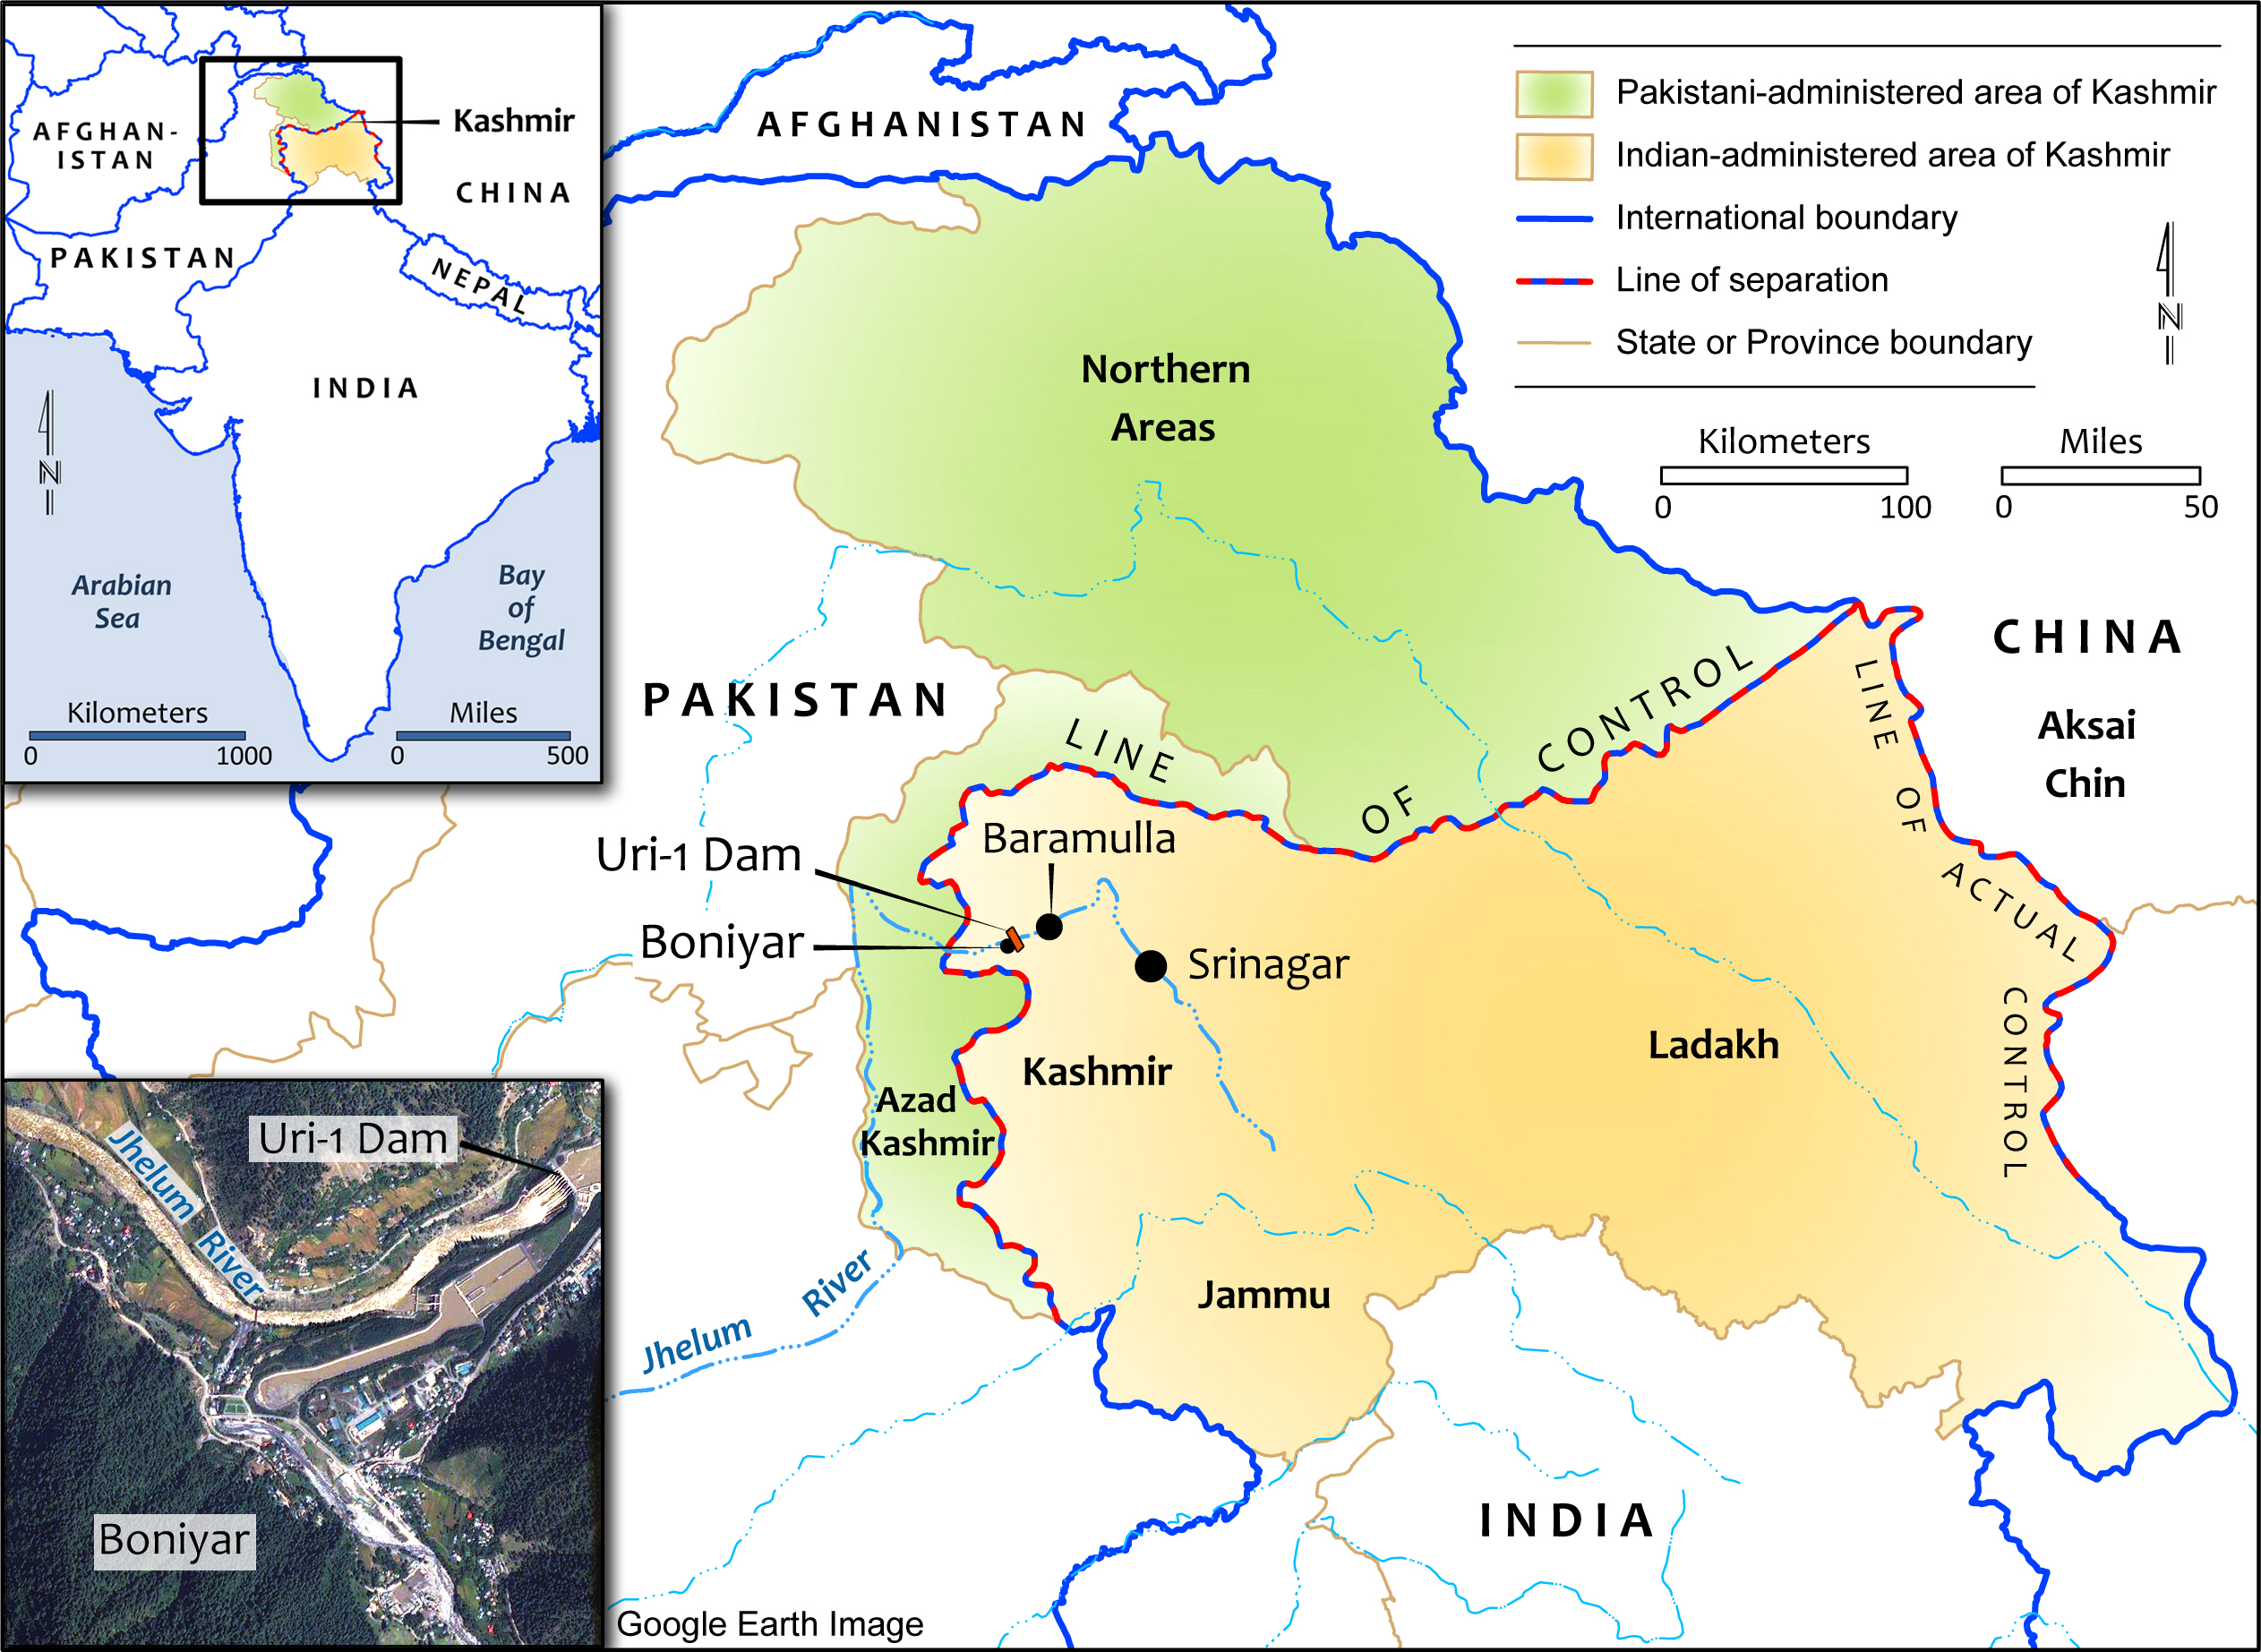
\includegraphics[width=\textwidth,height=0.8\textheight,keepaspectratio]{Kashmir.jpg}
\end{frame}

\begin{frame} 
\frametitle{\LARGE{The problem of anarchy}}
\begin{itemize}
    \item Example: Kashmir
    \begin{itemize} 
        \item Territory claimed by both India and Pakistan \pause
        \item Ceding the claim gives the other side a strategic advantage \pause
        \item Stakes are high due to historical claims \pause
        \item No authority above India and Pakistan to enforce a solution (or to prevent violent conflict over it) \pause
    \end{itemize}
    \item Deciding who gets what, how, and when becomes \textit{very} difficult without central authority
\end{itemize}
\end{frame}

\begin{frame} 
\frametitle{\LARGE{The main unit in international politics}}
\begin{itemize}
    \item \textbf{States} (``countries") are the primary actors in IR. \pause
    \item They are:
    \begin{itemize}
        \item central authorities \pause 
        \item with the ability to make laws, rules, and decisions \pause
        \item and enforce them via a monopoly on the use of violence \pause
        \item within a specified territory \pause
        \item recognized as sovereign by other states \pause
    \end{itemize}
    \item Because of their internal authority, they are an efficient way of deciding political problems within their borders.
\end{itemize}
\end{frame}

\begin{frame}{\LARGE Sovereignty}
\begin{itemize}
    \item Integral to the concept of the state is the principle of \textbf{sovereignty}. \pause
    \item \textbf{Sovereignty}: the expectation that states have legal and political supremacy and authority within their territorial borders.  \pause
    \begin{itemize}
    	\item Enforced by their monopoly on the use of force. \pause
    \end{itemize}
    \item The expectation is not always accurate (ex: failed states).  \pause
    \item But states (generally) presume each other to have sovereignty over affairs within their territory, with norms of non-intervention in the affairs of other states.
\end{itemize}
\end{frame}


\begin{frame}{\LARGE Brief Sidebar: State or Nation?}
\begin{itemize}
	\item What is the difference between a state and a nation? \pause
    \item \textbf{States} are tied to physical geography. \pause
    \item \textbf{Nations} are groups of people with common lineage, culture, or customs. \pause
    \item Nations may be confined to a single state, or be split across states. \pause
    \item States may contain many nations or be relatively homogeneous.
\end{itemize}
\end{frame}

\begin{frame}{\LARGE Bangladesh}
    \centering
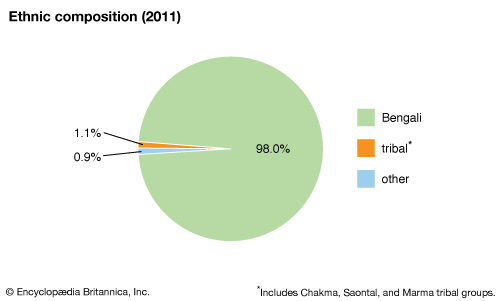
\includegraphics[width=\textwidth,height=0.8\textheight,keepaspectratio]{Bangladesh.jpg}
\end{frame}

\begin{frame}{\LARGE The Kurds}
    \centering
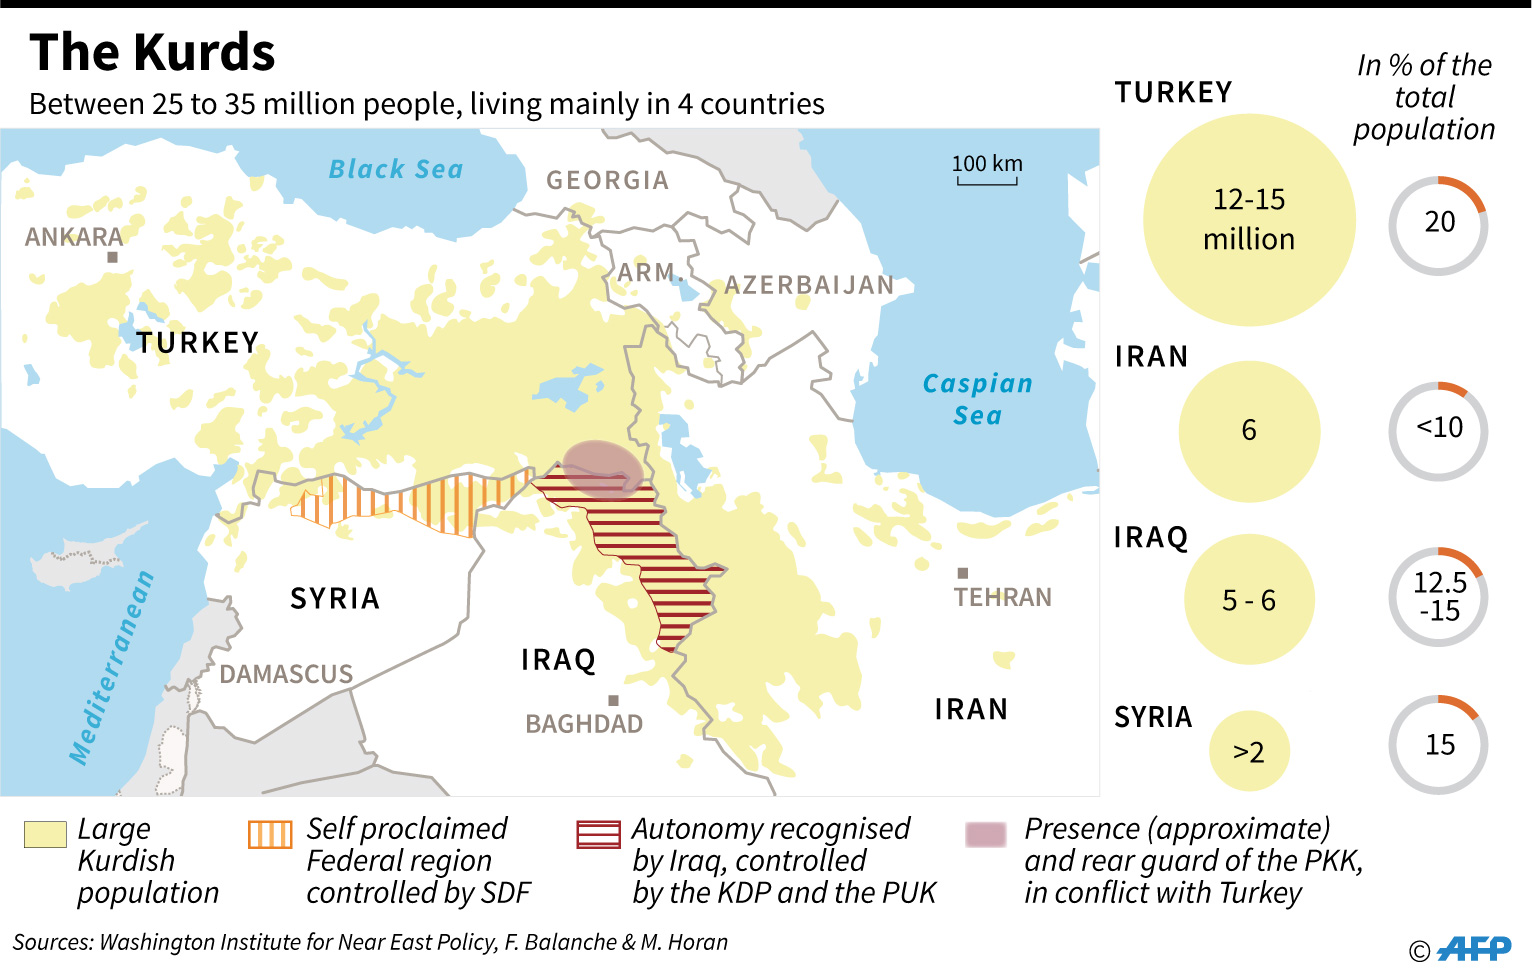
\includegraphics[width=\textwidth,height=0.8\textheight,keepaspectratio]{Kurds.jpg}
\end{frame}

\begin{frame}{\LARGE Africa}
    \centering
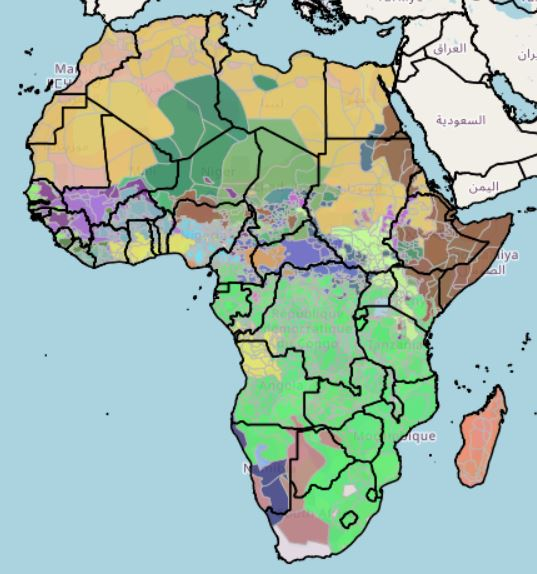
\includegraphics[width=\textwidth,height=0.8\textheight,keepaspectratio]{Africa.JPG}
\end{frame}

\begin{frame}{\LARGE Where did these concepts come from?}
\begin{itemize}
    \item We can trace the modern concept of the state and sovereignty to the outcome of the Thirty Years' War (1618-1648).  \pause
    \item Thirty Years' War (over-)simplified:
    \begin{itemize}
    	\item Holy Roman Emperor tries to establish Catholicism in Protestant regions within the empire.  \pause
    	\item This was an effort to establish central control over increasingly independent local principalities.  \pause 
    	\item This effort's primary objective: gain/retain tax revenues and loyalty from the people.  \pause
    	\item Local rulers violently disagreed.
    \end{itemize}
    \item War ends in \textbf{1648} with the \textbf{Peace of Westphalia}.
\end{itemize}
    
\end{frame}

\begin{frame}{\LARGE Peace of Westphalia}
\begin{itemize}
    \item Gives the princes control over the territory they confiscate from the Catholic Church and the Hapsburgs. \pause
    \item Allowed princes and their proto-states independent decision-making. \pause
    \item Establishes their authority over territories under their control, including defining specific borders for that control. \pause
    \item This means that control shifts from church and emperor to local units - these proto-states are now considered sovereign. \pause
    \item Citizens now give loyalty (and taxes) to their local states.
    \item Establishes importance of states and their sovereignty.
\end{itemize}
\end{frame}

\begin{frame}{\LARGE Peace of Westphalia Implications}
	\begin{itemize}
		\item Centuries later, this means that we often take for granted discussing why one state (ex: the US) behaves a certain way with another state (ex: China).
		\item We also tend to assume that all states possess the right to sovereignty and non-intervention.
		\item Think about how weird this is for a second. \pause
		\item There are (imaginary!) lines out in the world, where if you happen to live on one side of the line, your entire political life is controlled by one government, but if you live on the other side of the line, your political life may be totally different.
	\end{itemize}
\end{frame}

\begin{frame}{\LARGE PoW Implications: Who is ``the state"?}
	\begin{itemize}
		\item Who approved the Treaty of Westphalia? \pause
		\begin{itemize}
			\item Not ``the people,” but European rulers (mostly monarchs).
		\end{itemize}
		\item What did those rulers want? \pause
		\item Prior to Westphalia, rulers often had competing claims over which populations were their subjects (no clear borders). \pause
		\item This means they have to compete for citizens’ support, which can become very costly to do.
		\begin{itemize}
			\item This involves giving citizens more rights, more economic benefits, etc. (None of which rulers want to do!)
		\end{itemize}
		\item Economics shows that, when many firms compete for the same consumers, this is good for consumers but bad for firms.		
	\end{itemize}
\end{frame}

\begin{frame}{\LARGE PoW Implications: Who is ``the state"?}
\begin{itemize}
	\item What kind of arrangement shifts benefits away from consumers and to a firm? \pause
	\item Answer: Monopoly. \pause
	\item We can apply this to the post-PoW world. The clarification and settling of borders meant that rulers could focus on keeping their citizens in check, without needing to spend a bunch of extra resources competing against other monarchs for their citizens' support. 
	\item \textbf{This gives rise to the norms of sovereignty and non-interference.} 
\end{itemize}
\end{frame}


\begin{frame}{\LARGE PoW Implications: Who is "the state"?}
	\begin{itemize}
		\item Given that governments are sovereign, and not supposed to interfere with citizens in other states, \textbf{this lets us discuss the action of a state’s government as representing the interests of the state itself.} \pause
		\item HOWEVER: This is a useful fiction. States are always composed of many (sometimes competing) groups.
		\begin{itemize}
			\item Talking about a state's interests is a useful simplification of reality (most of the time).
			\item We'll return to this later...
		\end{itemize}
	\end{itemize}
\end{frame}


\begin{frame}{\LARGE Why are states so important?}
\begin{itemize}
     \item What does the origin of sovereignty mean for the state's relationship to war? 
    \\~\\
    \item How did this principle of state sovereignty spread to the rest of the world?
    \\~\\
    \item How does the tension between sovereignty and nations complicate politics?
\end{itemize}
\end{frame}

\begin{frame}{\LARGE Why are states so important?}
	\begin{itemize}
	     \item What does the origin of sovereignty mean for the state's relationship to war? \pause 
	    \begin{itemize}
	        \item War makes the state, and the state makes war (Tilly 1979). \pause
	        \item States use their monopoly on the legitimate use of force to impose peace within their territories, enabling them to efficiently tax. This tax revenue lets them maintain the military capacity to wage war on other states.
	    \end{itemize}
	    \item How did this principle of state sovereignty spread to the rest of the world? \pause
	    \begin{itemize}
	        \item Primarily through European imperialism. \pause
	    \end{itemize}
	    \item How does the tension between sovereignty and nations complicate politics? \pause
	    \begin{itemize}
	        \item Makes state control extremely valuable and worth fighting for, especially if two hostile nations are confined to one state.
	    \end{itemize}
	\end{itemize}
\end{frame}

\begin{frame}{\LARGE Historical Eras}
\begin{enumerate}
	\item The Mercantilist Era, 1492–1815
	\item The Pax Britannica, 1815–1914
	\item The Thirty Years’ Crisis, 1914–1945
	\item The Cold War, 1945–1990
	\item Post–Cold War, 1991–Present
	\item What Will Shape Our World in the Future?	
\end{enumerate}
\end{frame}

\begin{frame}{\LARGE The Mercantilist Era: 1492-1815}
 \centering
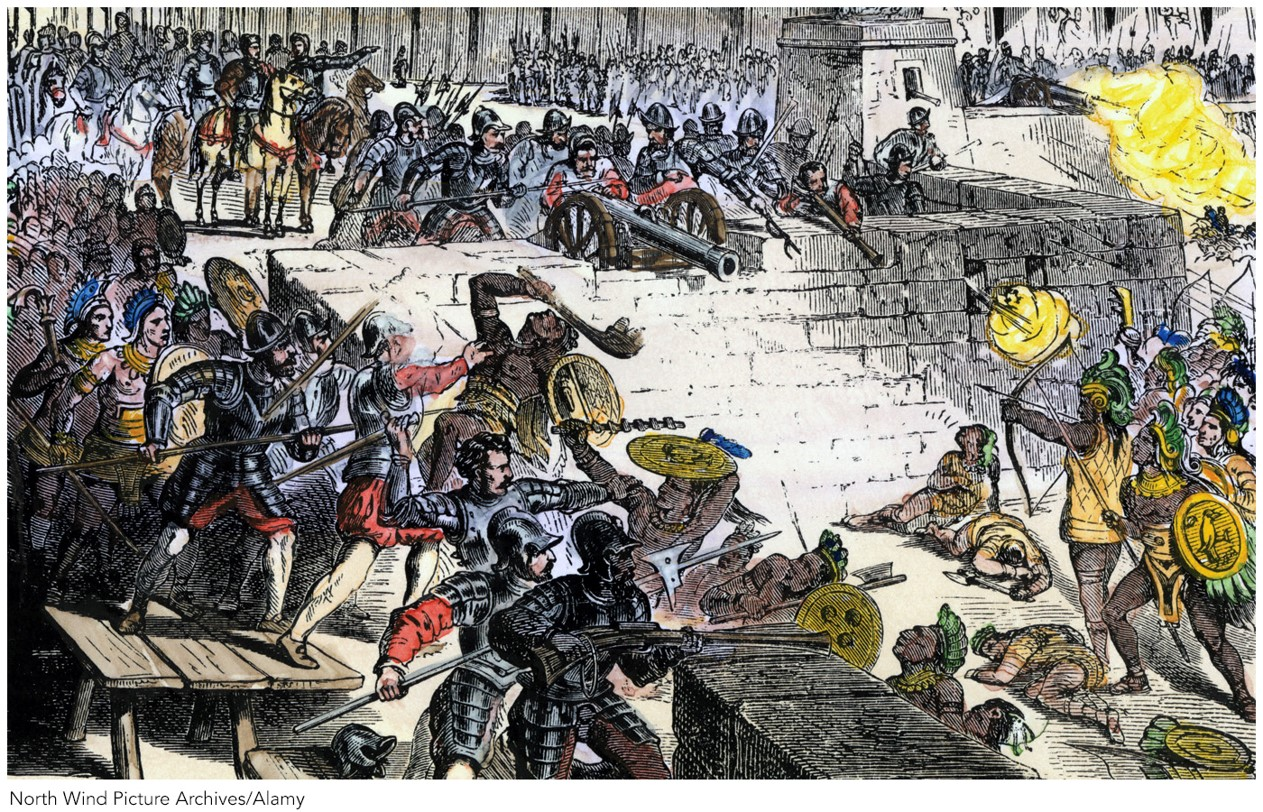
\includegraphics[width=\textwidth,height=.9\textheight,keepaspectratio]{Conquistadors.jpg}	
\end{frame}

\begin{frame}{\LARGE The Mercantilist Era: 1492-1815}
	\begin{itemize}
		\item The ``world” as a meaningful unit emerged after 1492.
		\item The Age of ``Discovery:" explorers such as Columbus (Spain) and Henry the Navigator (Portugal) traveled the world, and Spain and Portugal were the first to expand outward and to establish colonies abroad. \pause
		\item Prior slide image shows Spanish invaders in 1520 in Tenochtitlán, the site of modern-day Mexico City.
		\begin{itemize}
			\item Military technology, transportation (ships), and disease (e.g., blankets with smallpox) made conquest possible despite the relatively small numbers of Europeans. \pause
		\end{itemize}
		\item England, France, and the Netherlands promptly followed. 
	\end{itemize}
\end{frame}

\begin{frame}{\LARGE The Mercantilist Era: 1492-1815}
	\begin{itemize}
		\item Competition led the great powers to secure trade routes and establish colonial empires in the New World, Africa, and Asia. By 1700, Western European powers controlled much of the world.
		\item In this system, wealth and military power were mutually reinforcing.
		\item This led to \textbf{Mercantilism}: the use of military power to enrich imperial governments. This system intentionally favored the mother country over both its own colonies and competing empires.
	\end{itemize}
\end{frame}

\begin{frame}{\LARGE The Mercantilist Era: 1492-1815}
	\begin{itemize}
		\item Key mechanisms of mercantilism:
			\begin{itemize}
				\item State monopolies	
				\item Controls on colonial trade
		\end{itemize}	
		\item What does this mean in practice? \pause
		\item Goods made in colonies could only be exported to the imperial center, at prices substantially lower than those of world markets, while colonies could only purchase goods from that same center.
	\end{itemize}
\end{frame}

\begin{frame}{\LARGE The Mercantilist Era: 1492-1815}
	\begin{itemize}
		\item This leads to a battle for supremacy between rival imperial powers, who seek to colonize the rest of the planet to expand their own wealth via mercantilism.
		\begin{enumerate}
			\item Spain vs. Portugal for control of the ``New" World
			\item Spain’s possessions in the Netherlands rebelled in the 1560s and formed the New Dutch Republic.
			\item British and Spain battled in the late 1500s; Britain defeated the Spanish Armada in 1588.
			\item Thirty Years' War (1618-1648): French and Dutch vs. Spain (with other contributors). \textbf{Treaty of Westphalia}. \pause
		\end{enumerate}
		\item Does the Treaty of Westphalia bring peace to this era?
	\end{itemize}
\end{frame}

\begin{frame}{\LARGE The Mercantilist Era: 1492-1815}
	\begin{itemize}
		\item Of course not. \pause
		\item The following 150 years see a struggle for hegemony between England and France (and their respective allies).
		\item Notable conflicts
			\begin{itemize}
				\item Seven Years’ War (1756-1763): Cements British dominance in the New World (mostly).
				\item Napoleonic Wars (1804-1815): Establishes Britain as dominant force in Europe.				
			\end{itemize}
		\item Britain emerges as the \textbf{hegemon}: the undisputed superpower in the international system.
	\end{itemize}
\end{frame}


\begin{frame}{\LARGE The Pax Britannica: 1815-1914}
	\begin{itemize}
		\item Also called the ``Hundred Years' Peace"
		\item International cooperation generally encouraged by:
		\begin{itemize}
			\item Greater links among economies and governments.
			\item Less belligerent relations and converging interests.
			\item British hegemony and predominance (naval power) helping to maintain a rough power balance.
		\end{itemize}
	\end{itemize}
\end{frame}

\begin{frame}{\LARGE The Pax Britannica: 1815-1914}
	\begin{itemize}
		\item Exchange of goods and economic integration increase during this era, increasing GDP. Why? \pause
		\item Britain's Industrial Revolution: \pause
		\begin{itemize}
			\item Efficient, large-scale production by 1820s
			\item Rise of industrial and merchant class
			\item Mercantilism seen as harmful and inefficient \pause
		\end{itemize}
		\item New desire for free trade leads to trade liberalization in the 1880s.
		\item Transportation and communication grow too.
		\item Overall result: more free trade and migration, backed by the British gold standard (globalization v1).	
	\end{itemize}
\end{frame}

\begin{frame}{\LARGE The Pax Britannica: 1815-1914}
	\centering
	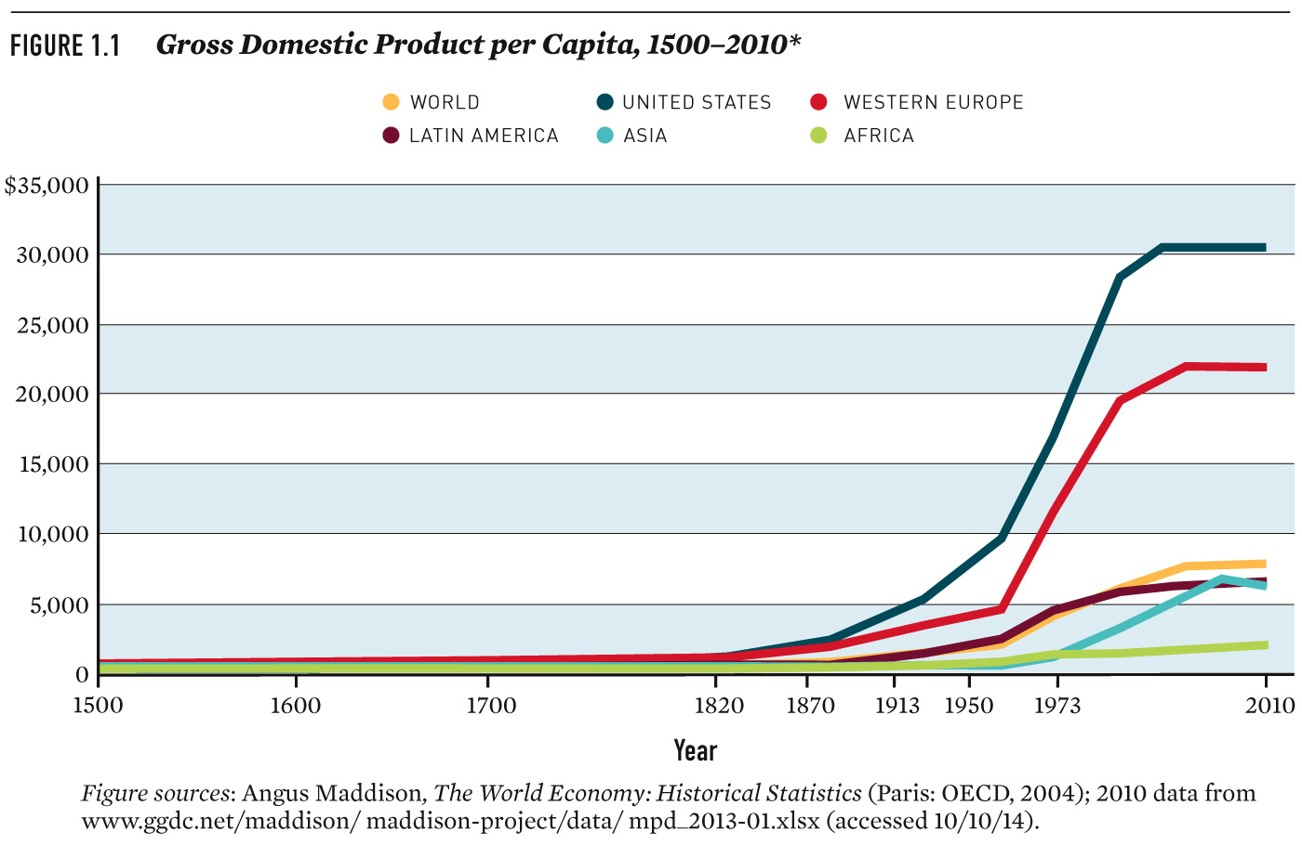
\includegraphics[width=\textwidth,height=.9\textheight,keepaspectratio]{500yearGDP.jpg}	
\end{frame}

\begin{frame}{\LARGE The Pax Britannica: 1815-1914}
	\centering
	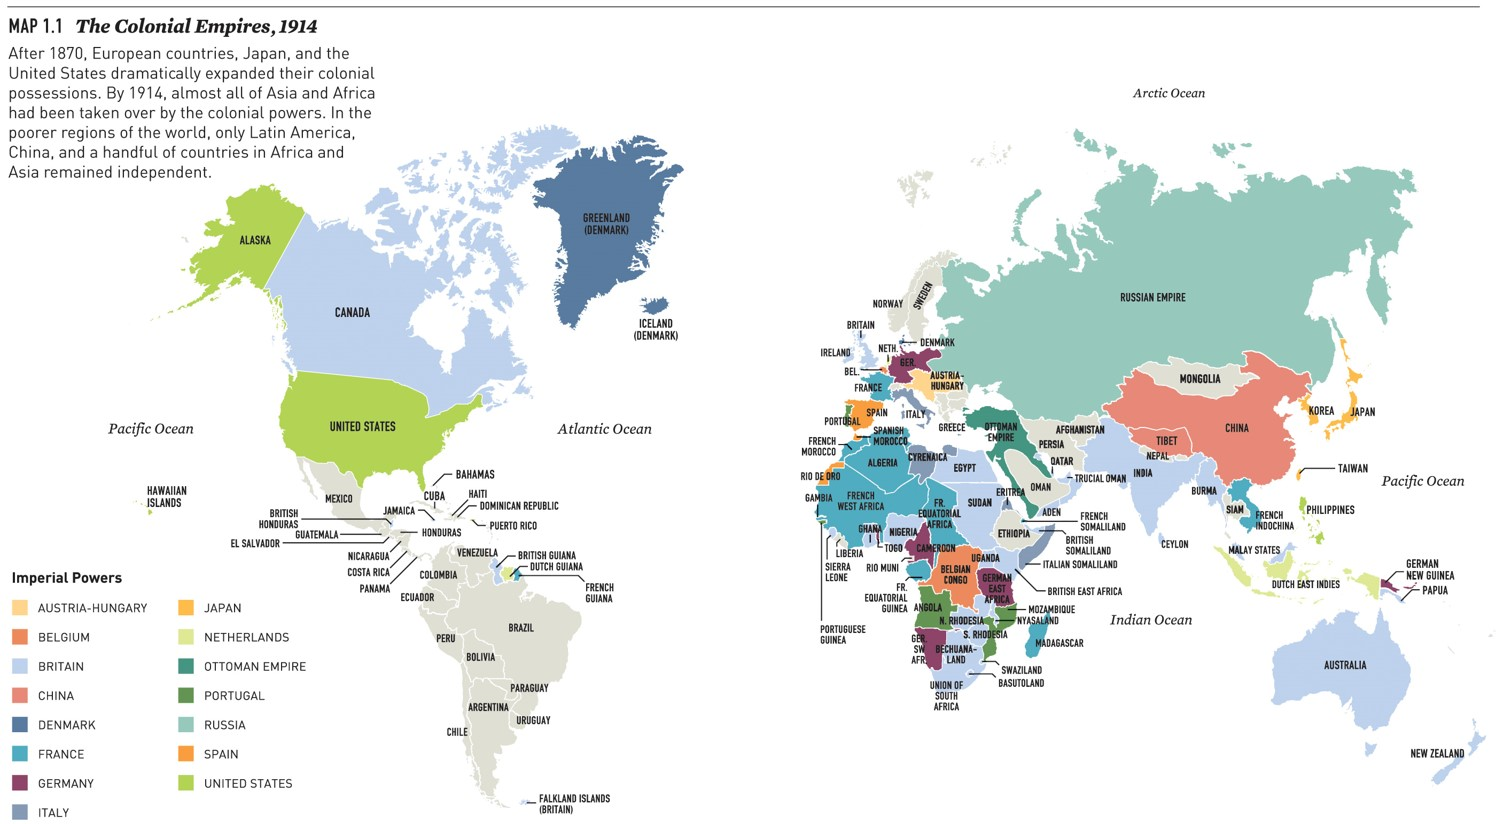
\includegraphics[width=\textwidth,height=.9\textheight,keepaspectratio]{Colonialempires1914.jpg}	
\end{frame}

\begin{frame}{\LARGE The Thirty Years' Crisis: 1914-1945}
	\begin{itemize}
		\item States generally wanted security through alliances, expansion, and economic self-sufficiency. \pause
		\item Rising powers (particularly Germany and Japan) chafed at “established” political boundaries, believing that they were being artificially restrained. \pause
		\item Over time, relations became more conflictual.	Europe divides into two camps: Central versus Allied powers.		
	\end{itemize}
\end{frame}

\begin{frame}{\LARGE The Thirty Years' Crisis: 1914-1945}
	\centering
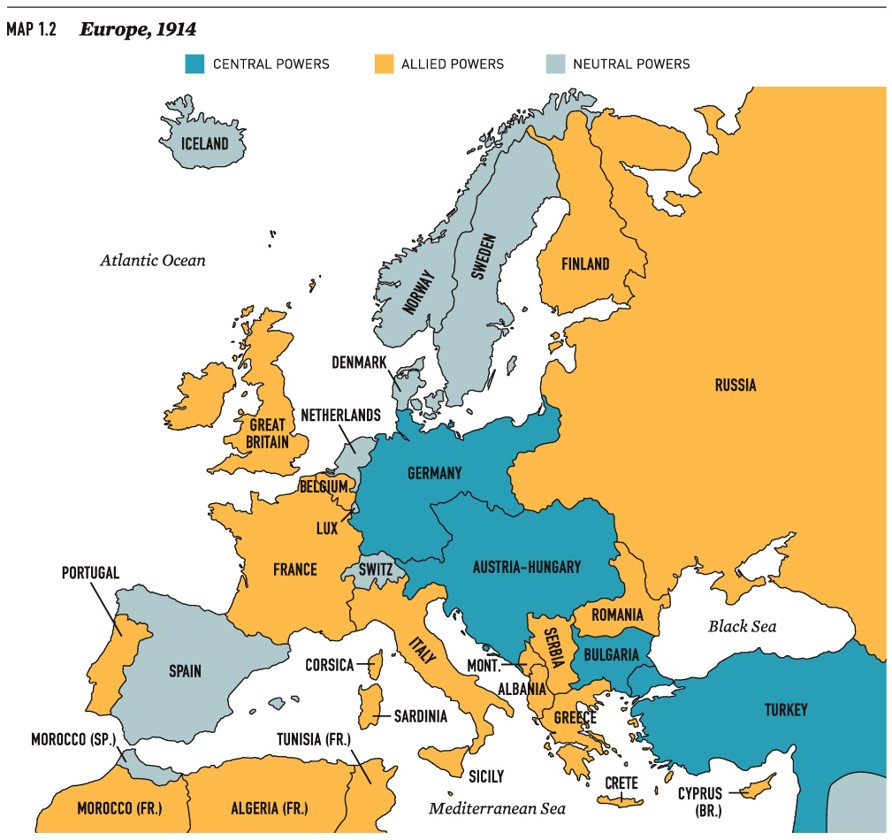
\includegraphics[width=\textwidth,height=.9\textheight,keepaspectratio]{CentralandAlliedpowers1914.jpg}
\end{frame}

\begin{frame}{\LARGE The Thirty Years' Crisis: World War I}
	\begin{itemize}
		\item World War I: Costly and bloody war of attrition. Ultimately decided by late US entry (1917) and inability of German submarines to cut off British supplies.
		\item Assorted consequences: Central powers defeated, Russian Revolution and Soviet Union formation, new states replaced Austro-Hungarian and Ottoman empires.
	\end{itemize}
\end{frame}

\begin{frame}{\LARGE The Thirty Years' Crisis: 1914-1945}
	\centering
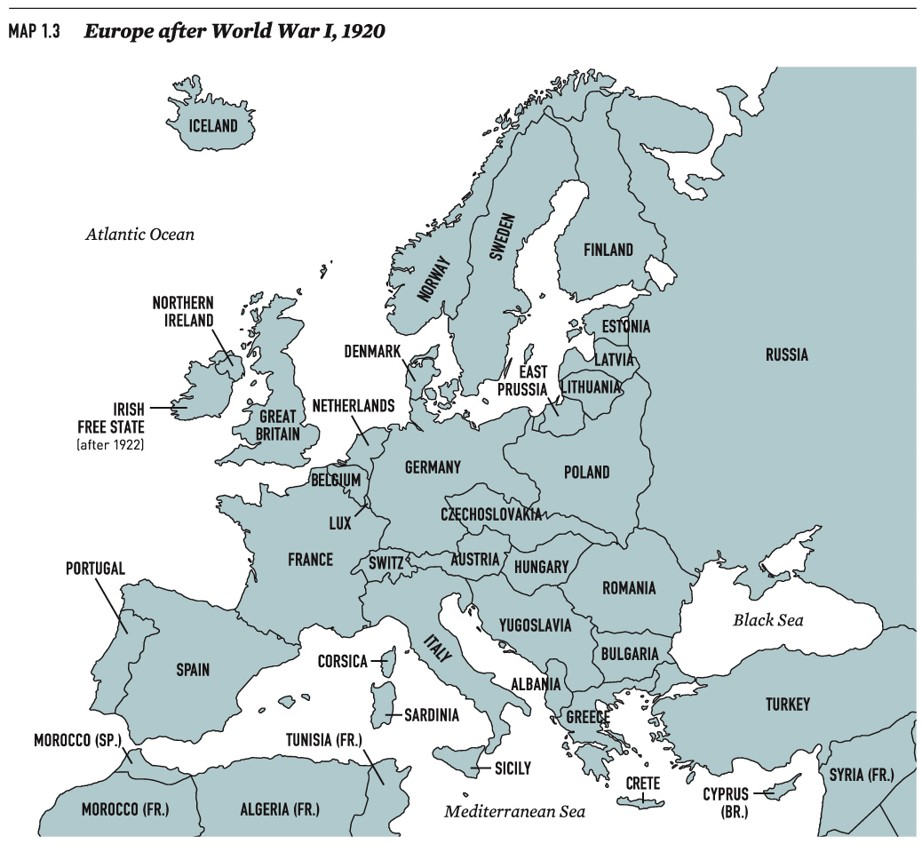
\includegraphics[width=\textwidth,height=.9\textheight,keepaspectratio]{Europe1920.jpg}
\end{frame}

\begin{frame}{\LARGE Treaty of Versailles}
	\begin{itemize}
		\item The Treaty of Versailles, June 1918.
		\item Punishes Germany as WWI's aggressor, leading to loss of territory and status.
		\item Forces Germany to pay war reparations to Allied countries to cover their costs of going to war.
		\begin{itemize}
			\item Many of these costs were actually to pay loans to the US, which had made loans available during the war to allow these states to afford huge military expenditures.
		\end{itemize}
		\item German economy could not afford both reparations and rebuilding.
		\item This leads to the government printing more and more money…		
	\end{itemize}
\end{frame}

\begin{frame}{\LARGE The Thirty Years' Crisis: Hyperinflation}
	\begin{figure}
		\centering
		\begin{subfigure}{0.49\textwidth}
			\centering
			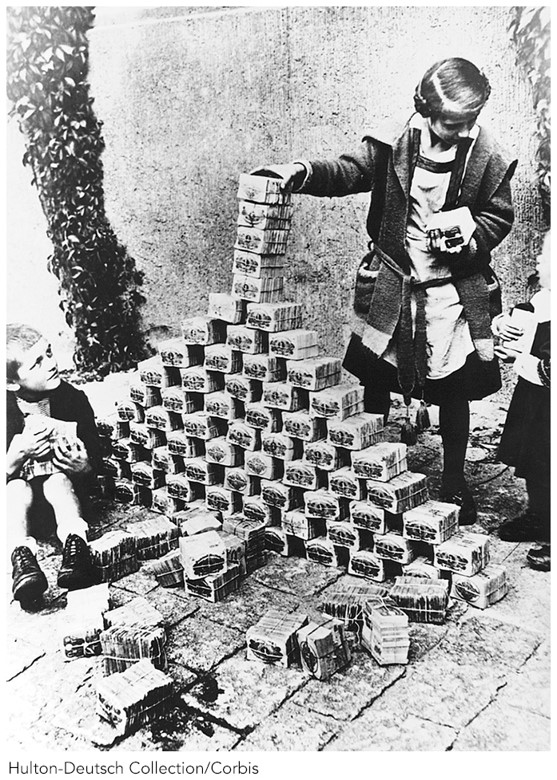
\includegraphics[width = \textwidth,height=.9\textheight]{Deutschmarkpiles.jpg}
		\end{subfigure}
		\begin{subfigure}{0.49\textwidth} %this is actually hitler vs unemployment
			\centering
			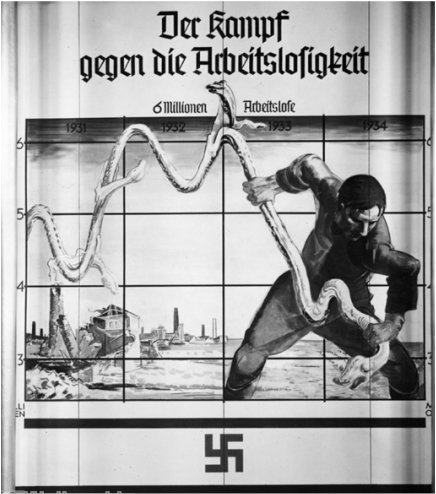
\includegraphics[width = \textwidth, height=.9\textheight]{Hitlervsinflation.png}
		\end{subfigure}
	\end{figure}
\end{frame}

\begin{frame}{\LARGE The Thirty Years' Crisis Continued}
	\begin{itemize}
		\item 1929: Great Depression. This has global economic impacts.
		\begin{itemize}
			\item U.S. industrial production drops by half.
			\item One-third of the labor force is unemployed in Germany.
			\item Free trade ends; the volume of world trade drops 67\% between 1929 and 1933.			
		\end{itemize}
		\item States turn inward with more protectionism and decreased trade; fascism and imperialism on the rise.
	\end{itemize}
\end{frame}


\begin{frame}{\LARGE The Thirty Years' Crisis: WWII}
	\begin{itemize}
		\item WWII: Germany invades Poland and the war begins.
		\item Axis Powers: Germany, Italy, Japan.
		\item Allied Powers: US, Britain, USSR
		\item US and USSR left standing as only viable superpowers; widespread devastation in Europe.
	\end{itemize}
\end{frame}

\begin{frame}{\LARGE The Cold War: 1945-1991}
	\begin{itemize}
		\item Superpowers form alliances and gather allies while trying to maximize global influence and regrow their economies.
	\end{itemize}
\end{frame}

\begin{frame}{\LARGE The Cold War: 1945-1991}
	\centering
	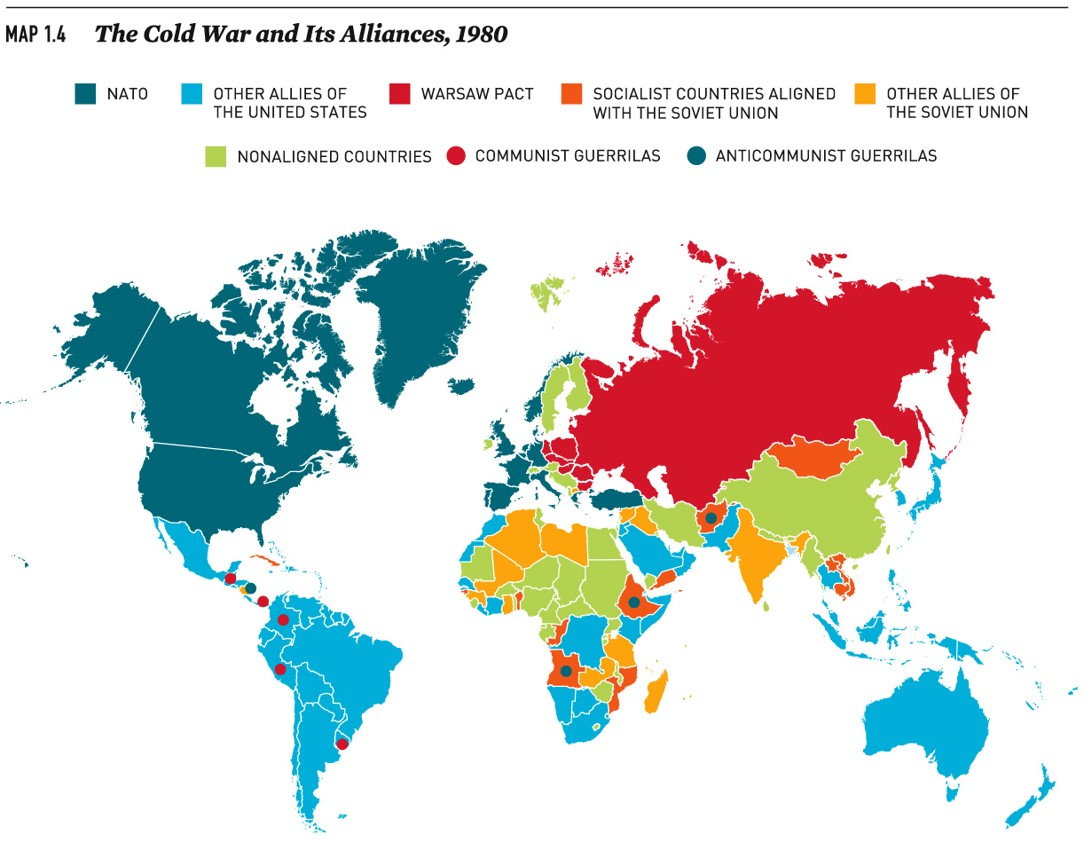
\includegraphics[width=\textwidth,height=.9\textheight,keepaspectratio]{ColdWar1980.jpg}
\end{frame}

\begin{frame}{\LARGE The Cold War: 1945-1991}
	\begin{itemize}
		\item Rise of the ``third world" (more recently called ``Less Developed Countries").
		\item Most of the dominant countries were preoccupied with war or rebuilding from 1915-1960.
		\item This meant that many colonial areas were neglected, leading to pressure for independence.
		\item This generates a huge wave of “de-colonization;” almost all colonial powers have given up their colonies by late 1960s.
		\item Now, the world was composed of sovereign states rather than empires.
	\end{itemize}
\end{frame}

\begin{frame}{\LARGE The Cold War: 1945-1991}
	\begin{itemize}
		\item Eventually, rising costs to Soviet economy of competition with US leads to attempts at political and economic reform (Gorbachev's glasnost and perestroika).
		\item These prove insufficient...		
	\end{itemize}
\end{frame}

\begin{frame}{\LARGE Post-Cold War: 1991-Present}
\centering
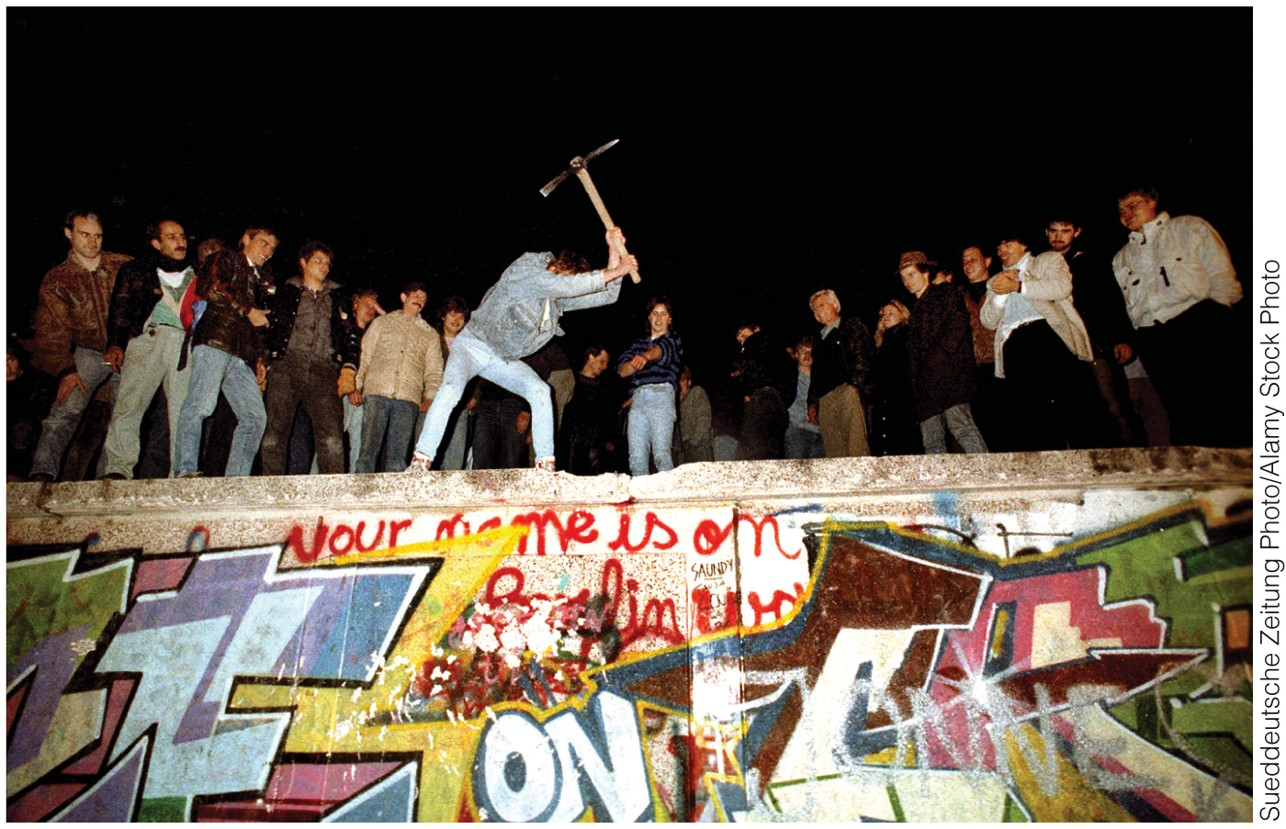
\includegraphics[width=\textwidth,height=.9\textheight,keepaspectratio]{Berlinwall.jpg}
\end{frame}

\begin{frame}{\LARGE Post-Cold War: 1991-Present}
	\begin{itemize}
		\item USSR collapses due to a number of factors:
		\begin{itemize}
			\item The Soviet economy lags behind the West.
			\item Gorbachev seeks better relations with the West.
			\item Glasnost and perestroika decrease state control.
			\item Soviets leave Afghanistan in 1989 after 10 years of fighting.
		\end{itemize}
		\item Soviet Union becomes 15 separate states; Eastern European states hold elections.
	\end{itemize}
\end{frame}

\begin{frame}{\LARGE Post-Cold War: 1991-Present}
	\begin{itemize}
		\item Increase in international cooperation: cooperation in the 1991 Gulf War.
		\item Increased United Nations peacekeeping and global role.
		\item Increased global economic integration, interdependence, and institutions (although multiple financial crises also occurred).
	\end{itemize}
\end{frame}

\begin{frame}{\LARGE Post-Cold War: 1991-Present}
\centering
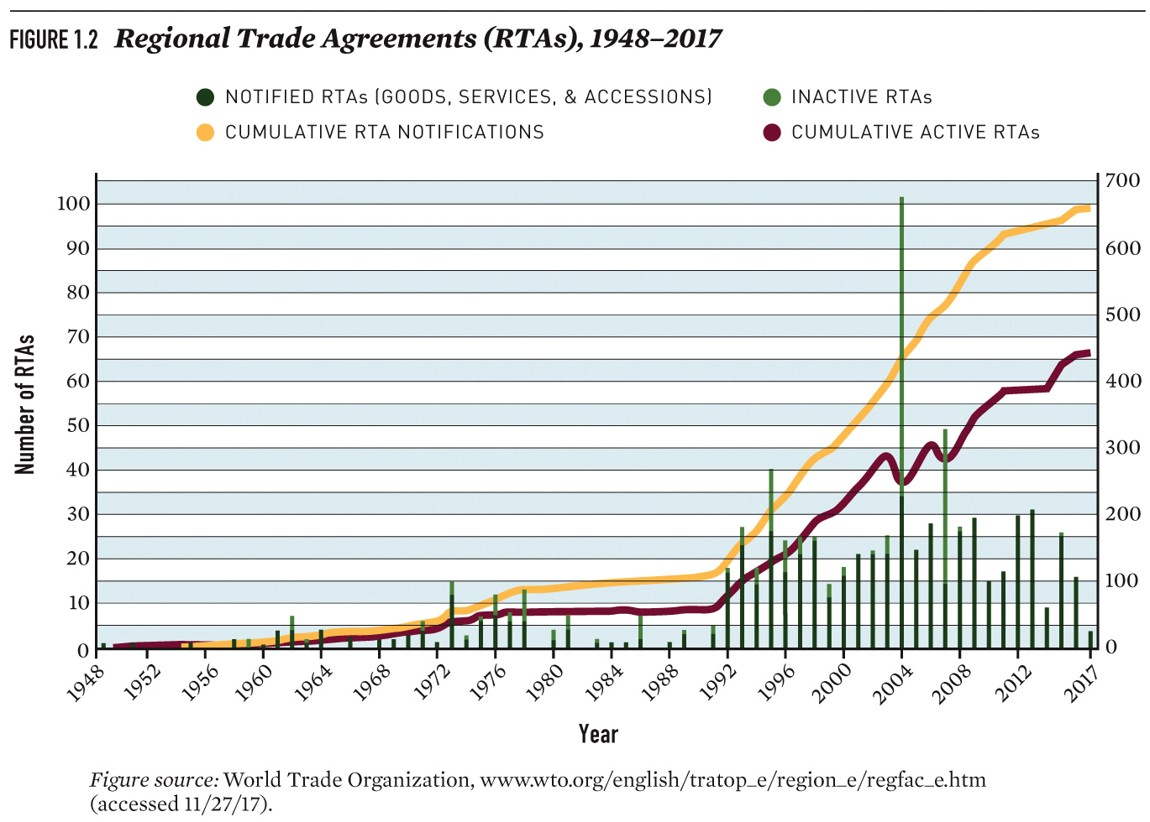
\includegraphics[width=\textwidth,height=.9\textheight,keepaspectratio]{RTAs.jpg}
\end{frame}

\begin{frame}{\LARGE Post-Cold War: 1991-Present}
	\begin{itemize}
		\item This era has not been without crises.
		\begin{itemize}
			\item 1990 Iraq invasion of Kuwait
			\item 1992 UN mission in Somalia 
			\item 1993 Rwandan genocide
			\item 9/11 and the War on Terror
			\item 2011: Arab Spring and its aftermath
			\begin{itemize}
				\item ISIS in Syria, Iraq, Libya, Afghanistan
				\item Civil war in Yemen
				\item Massive refugee flows to Europe and reactionary formation of anti-immigrant parties
			\end{itemize}	
		\end{itemize}
	\end{itemize}
\end{frame}

\begin{frame}{\LARGE Future Challenges}
	\begin{itemize}
		\item Diplomatic
		\begin{itemize}
			\item Yemen civil war
			\item Chinese territorial claims
			\item North Korean nuclear power
			\item Russian annexation of Crimea and invasion of Ukraine \pause
		\end{itemize}
	\end{itemize}
	\begin{itemize}
		\item Economic
		\begin{itemize}
			\item Inequality
			\item Decreased support for globalization
			\item Rise in populism
			\item Covid impacts (social, financial, etc.)
			\item America's role in and commitment to its alliances			
		\end{itemize}
	\end{itemize}
\end{frame}

\begin{frame}{\LARGE How do states interact?}
\begin{itemize} 
	\item In this history, we can see a variety of international orders. \pause
    \item \textbf{International order:} the governing arrangements among a group of states; the rules, principles, and institutions that guide their actions towards each other \pause
    \item We can generally classify at least three types of international order.
\end{itemize}
\end{frame}

\begin{frame}{\LARGE Varieties of international order}
\begin{itemize}
    \item \textbf{Multipolar}: A variety of (groups of) states of roughly equal strength vie for power. \pause
    \item \textbf{Bipolar}: Two states of equal strength balance each other's power, often collecting weaker states into alliances. \pause
    \item \textbf{Hegemonic}: One state with disproportionate strength makes and enforces its own rules.
    
\end{itemize}
\end{frame}

\begin{frame}{\LARGE Broad international orders since 1492}
	\begin{itemize}
		\item \textbf{The Mercantilist Era:} \pause Mixture of multipolar (Spain vs. others) and bipolar (England vs. France). \pause
		\item \textbf{Pax Britannica:} \pause Mostly hegemonic (Britain). \pause
		\item \textbf{30 Years' Crisis:} \pause Multipolar.
		\item \textbf{Cold War:} \pause Bipolar (US vs. USSR). \pause
		\item \textbf{Age of Globalization to present:} \pause Briefly hegemonic (US 1991 onwards to mid-2000s) then shift towards multipolarity (US, Russia, China, EU).
		\item \textbf{2022 and beyond:} \pause Increasing multipolarity? 
	\end{itemize}
\end{frame}

\end{document}
